\documentclass[runningheads,a4paper]{llncs}

\usepackage{amssymb}
\setcounter{tocdepth}{3}
\usepackage{graphicx}
\usepackage{booktabs}

\usepackage{url}
\urldef{\mailsa}\path|{alfred.hofmann, ursula.barth, ingrid.haas, frank.holzwarth,|
\urldef{\mailsb}\path|anna.kramer, leonie.kunz, christine.reiss, nicole.sator,|
\urldef{\mailsc}\path|erika.siebert-cole, peter.strasser, lncs}@springer.com|
\newcommand{\keywords}[1]{\par\addvspace\baselineskip
\noindent\keywordname\enspace\ignorespaces#1}

\begin{document}

\mainmatter  % start of an individual contribution

% first the title is needed
\title{Distributed Programming in Cloud Computing Platforms}

% a short form should be given in case it is too long for the running head
\titlerunning{Information Systems and Computer Engineering}

% the name(s) of the author(s) follow(s) next
%
% NB: Chinese authors should write their first names(s) in front of
% their surnames. This ensures that the names appear correctly in
% the running heads and the author index.
%
\author{Enes Uysal – 72560}
%\thanks{Please note that the LNCS Editorial assumes that all authors have used
%the western naming convention, with given names preceding surnames. This determines
%the structure of the names in the running heads and the author index.}%
%\and Ursula Barth\and Ingrid Haas\and Frank Holzwarth\and\\
%Anna Kramer\and Leonie Kunz\and Christine Rei\ss\and\\
%Nicole Sator\and Erika Siebert-Cole\and Peter Stra\ss er}
%
\authorrunning{}
% (feature abused for this document to repeat the title also on left hand pages)

% the affiliations are given next; don't give your e-mail address
% unless you accept that it will be published
\institute{Departamento de Engenharia Informática\\
Instituto Superior Técnico\\
}

%
% NB: a more complex sample for affiliations and the mapping to the
% corresponding authors can be found in the file "llncs.dem"
% (search for the string "\mainmatter" where a contribution starts).
% "llncs.dem" accompanies the document class "llncs.cls".
%

\toctitle{Lecture Notes in Computer Science}
\tocauthor{Authors' Instructions}
\maketitle


\begin{abstract}
In Cloud environment, distributed programming solutions which cover interoperability between heterogeneous systems are essentially based on SOA or REST technology that uses HTTP, XML and JSON. These technologies are not developed for distributed programming in cloud computing environment to develop distributed applications, they were developed in the Web context for the integration of existing systems.\\

SOA and Web services are heavy and complex technologies. REST is more simple than SOA, but none of them is not very efficient, based on HTTP and  text-based data description languages (XML and JSON). The binary version of XML is no more than a compression data only for transmission effect (compressed and decompressed on the issue at the reception). A solution used in this work uses binary data format natively and does not require schema and uses Web Sockets as the runtime environment and these Web Sockets are much more efficient than HTTP, while maintaining some compatibility.\\

New solution is developed for distributed programming in cloud computing environment to develop distributed applications. While this solution compared with classical solution which is based on SOA and REST, this solution uses asymmetric interoperability which is based on compliance and conformance. The aim of this work is to explain this solution and its execution environment and also to compare it with the corresponding solution technologies which are based on SOA (Web Services) and REST.

\keywords{SOA, WSDL, REST, XML, JSON, HTTP, Web Sockets}
\end{abstract}


\section{Introduction}

Distributed applications are required in most of central application sectors including e-commerce, e-banking, e-learning, e-health, telecommunication and transportation\cite{introduction1}. In distributed applications that share information between each other does not need to be built with same technologies. The fundamental problem is the programming of distributed applications with all the basic interoperability problems involving distributed platforms and heterogeneous components. Clouds is a new challenge for distribution. They also create distributed platforms and that’s why they need to be able to support distributed applications as easily as possible. That’s make importance of interoperability in cloud environment because different cloud providers can have different properties and they need to communicate between each other.\\

The traditional integration technologies are based on either SOA or REST and they use the document concept as the foundation, with a data description language as the representation format and schema sharing as the interoperability mechanism (both sides use the same schema such XML Schema) or using previously known data types. The solutions for SOA or REST were also based on text (XML or JSON) and use connectionless protocol (HTTP).

The main problem of the traditional integration technologies creates coupling between the provider and the consumer, because both customer and provider are forced to implement full interoperability (for example, sharing a XML schema). This leads to a greater coupling than needed. Another problem is using XML or JSON to solve data interoperability, which is inefficient in computer terms due to parsing data to build a DOM tree and validating schemas to validate structure of message.
The main problems with using traditional integration technologies can be summerized as follows:
\begin{itemize}
  \item Data interoperability problems based on XML and JSON (Stub generation,DOM parsing)
  \item Service interoperabiliy problems based on SOA and REST(Coupling with schema sharing)
  \item The underlying protocol, usually HTTP, without binary support
\end{itemize}

New solution provides the maximum decoupling possible while ensuring the minimum interoperability requirements and allowing the client or the sender to changebility, as long as the actually used parts do not change. The interoperability is handled using compliance(consumer must satisfy the requirements established by the provider to accept requests sent to it)\cite{compliance} and conformance(the provider must fulfill the expectations of the consumer regarding the effects of a request)\cite{comformance} instead of sharing the same schema. Another solution for performance instead of using XML or JSON, based on text which is heavy and hard to parse, using binary directly for message transportation which reduce complexity improve performance. Again for performance, regarding message transportation, using Web Sockets and HTTP/2 protocol (a binary protocol with small message frames) instead using classical HTTP.

\section{State-of-the-art}

Web services allow you to use two different machines or two different pieces of code that talk each other. Two different applications can talk to each other over the network. They can call methods of each other over the network by using web service technology. The other advantage of using web services is that actually it is a standard technology because it is not really specific to Java or any other language. You can write web services using all other technologies. There are primarily two different types of web services. One of these types called as Simple Object Access Protocol (SOAP) web service and another type called as REpresentational State Transfer(REST) web service.

Simple Object Access Protocol, or SOAP as it was the first attempt to standardize a web service interface. It is based on sending an XML message to a service, in a specific XML format, and receiving an XML response in another specific format. This XML document is actually called as WSDL(Web Services Description Language)\cite{state3}. As an example, when you are sending any information across the network from a client to the web services and return type back to the client, the data has to be in XML format. You are not really sending Java string or Java object. So it has to be language natural format which is XML. There is specification about how you need to send all these different types. It is a protocol that is a way in which both sender and receiver use and this XML is called SOAP(Simple Object Access Protocol). It is a way in which these different technologies can access objects can access data. The message can be sent across different transports, including HTTP, FTP (File transfer Protocol), SMTP (Simple Mail Transfer Protocol) and more\cite{state2}. The specification does not dictate the transport over which the message should be sent, but most implementations send the XML message over HTTP.

REST (Representational State Transfer) was created in 2000 by Roy Fielding\cite{state5_1}. Developed in an academic environment, this protocol embraces the philosophy of the open Web. Instead of using XML to make a request, REST relies on a simple URL in many cases. In some situations you must provide additional information in special ways, but most Web services using REST rely exclusively on obtaining the needed information using the URL approach. REST can use four different HTTP 1.1 verbs (GET, POST, PUT, and DELETE) to perform tasks.

Everything in REST web services has URl is unique and standard. For example Facebook, when you open an account on Facebook, you will get a profile page that obivously dynamically generated pages, so whenever there is a new profile, it basically the same page which does same processing but render different content depending on profile that you are watching. In REST web services you need to think of resources and create unique URls for them. For example you are creating weathercast application and you want to get weather for different cities of Portugal, so your URl needs to be unique for each city as in table \ref{tab:urlexample}.

\begin{table}[!htb]
  \renewcommand{\arraystretch}{1.2} % more space between rows
  \centering
  \begin{tabular}{lccc}
    \toprule
    URl & Description  \\
    \midrule
    http://weatherapp.com/city/Lisbon &  Unique URl for Lisbon city\\
    http://weatherapp.com/city/Porto & Unique URl for Porto city\\
    http://weatherapp.com/city/Algarve & Unique URl for Algarve city\\
    \bottomrule
  \end{tabular}
  \caption[URl Example.]{URl Example.}
  \label{tab:urlexample}
\end{table}

The contents of messages in distrubuted systems need to be serialized to be sent over the channel and the format to do so (such as XML or JSON). The serialization formats used in the Web (e.g., XML, JSON) are text-based and thus verbose and costly in communications. Technologies have been developed to compress text-based documents\cite{state5_3}, such as EXI (Efficient XML Interchange), BSON and others\cite{state5_4}. However, these are compression technologies, which need text parsing after decompression.

In spite of the differences, both suffer from drawbacks and limitations: They are text based, which means inefficient parsing and data traversal where all characters of a component need to be parsed to reach the next one, high memory consumption, relevant message transmission times and poor support for binary data.

HTTP/2 is the second major version of the HTTP network protocol used by the World Wide Web. HTTP/2 will make our applications faster, simpler, and more powerful. The primary goals for HTTP/2 are to reduce latency by enabling full request and response multiplexing, minimize protocol overhead via efficient compression of HTTP header fields, and add support for request prioritization and server push\cite{state10}.

HTTP/2 breaks down the HTTP protocol communication into an exchange of binary-encoded frames, which are then mapped to messages that belong to a particular stream, and all of which are multiplexed within a single TCP connection. HTTP/2 communication is split into smaller messages and frames, each of which is encoded in binary format. This is the foundation that enables all other features and performance optimizations provided by the HTTP/2 protocol.

WebSockets\cite{matching} are a relatively new technology which promises to make websites more reactive by allowing lower latency interaction between users and the server. WebSockets circumvent some of the limitations of HTTP which removes this restriction, adds binary support and increases performance.

WebSocket is a protocol which allows for communication between the client and the server/endpoint using a single TCP connection. it sounds a bit like HTTP. The advantage WebSocket has over HTTP is that the protocol is full-duplex (allows for simultaneous two-way communcation) and it’s header is much smaller than that of a HTTP header, allowing for more efficient communcation even over small packets of data.

\section{Interoperability}
Resources need to interact to accomplish collaboration, that’s why Interoperability, a necessary condition to achieve integration between different systems. Another important factor for integration between systems is decoupling which says that resources need to be independent to evolve freely and dynamically. Unfortunately, independent resources do not understand each other and are not able to interact. Therefore, the fundamental problem of resource integration is to provide the maximum decoupling possible while ensuring the minimum interoperability requirements.

Currently, enterprise integration is based on SOA with Web Services and REST with HTTP.  These styles use symmetric arrangement in which a sender produces a message according to some schema and the receiver uses the same schema to validate and to get the contents of the message. In SOA web services, schema is usual in XML Schema and WSDL. In the REST world, schemas are known as media types but perform the same role. In any case, the schema or media type must be the same at both sender and receiver and therefore imposes coupling between the resources for all its possible values, even if only a few are actually used. In either case, data types need to be fully known by both interacting resources. Resources send requests to each other to invoke a given operation with a SOA or REST approach. These requests and their responses usually contain data, which is serialized, sent and reconstructed upon reception of the corresponding message. Most used data types for SOA and REST are XML and JSON. Both XML and JSON are text based which means inefficient parsing and all characters of a component need to be parsed to reach the next one. When using XML, there is a need to work with this document to understand message, which is sent by server or client side. The solutions are exist for that, are Databinding, DOM (Document Object Model) or SAX (Simple API for XML)\cite{arch20}. In these technologies, both customer and provider are forced to implement full interoperability (for example, sharing a XML schema), even if only a fraction of the possible interactions is used. This leads to a greater coupling than needed. In the next section, the proposed solution reduces coupling with using partial interoperability and creating the maximum decoupling possible while ensuring the minimum interoperability requirements.
\section{Architecture of the solution}
In the new implemented solution, it is showed that how interaction is still possible with only a partial knowledge of types, as long as the characteristics actually used are included (partial interoperability). This is a way of getting closer to solving the fundamental integration problem, by reducing coupling to what is actually required.

In this solution, a different approach will be showed, based on compliance. Messages do not obey some external schema. Each message has one specific value, which are structured or primitive with its own exclusive schema that is nothing more than a self-description, without the value variability that a type exhibits. This value and its description can be validated against an infinite number of schemas, those that have this particular value included in the set of their instances.
The receiver in figure~\ref{fig:Asymmetric} exposes a schema that defines the values it is willing to accept. When a message is received, its internal schema is checked against the receiver’s own schema. If it complies which means satisfies all the requirements of the receiver’s schema, the message can be accepted and processed. The advantage of this is that a resource can send a message to all the resources with schemas that the message complies with and, conversely, a resource can receive messages from any resource that sends messages compliant with its receiving schema. In other words, coupling occurs only in the characteristics actually used by messages and not in all the characteristics of the schemas used to generate the message or to describe the service of the receiving resource. Since the schemas of the message and of the receiver are not agreed beforehand, they need to be checked structurally. Sender and receiver no longer need to be designed for each other but, as long as compliance is ensured, one resource can replace another. In this case, what is involved is conformance between the replacement and the resource replaced, stating that the former supports all the characteristics supported by the latter. When a resource is able to interact with another, although not entirely interoperable with it, it means that there is partial interoperability.
\begin{figure}[!htb]
 \centering
 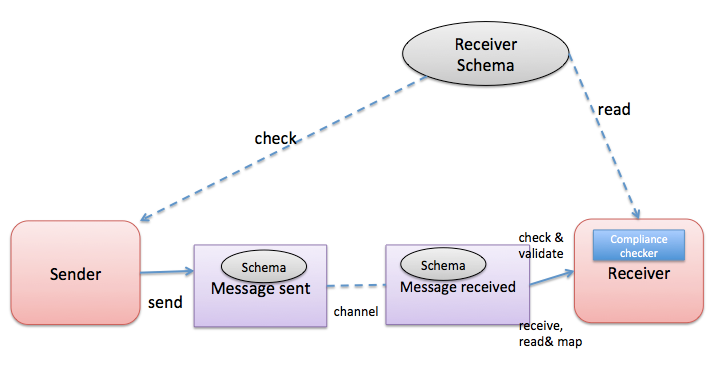
\includegraphics[width=0.9\textwidth]{Figures/asyc.png}
 \caption[Asymmetric interoperability.]{Asymmetric interoperability.}
 \label{fig:Asymmetric}
\end{figure}

One of ideas in this technology is using binary format instead of using text or other formats. Because binary is faster to write, communicate and read. When serialization or deserialization performance is compared with binary, XML and JSON, it is easily seen that binary format gives faster speed than the others especially with large data\cite{binaryOnline}.
Defining a binary format which messages are serialized on send and recovered on reception. For binary format using TLV (Tag, Length and Value) binary markup\cite{asn1}, array of bytes are used with each resource serialized in a tag (a byte codifying each resource type), size, name (only on structure and resource components) and value (the actual sequence of bytes resulting from serializing the resource).
\section{Implementation}
In the implemeted solution, compliance is done at the binary level, with primitive components. It is done both formal argument of the receiver method and received message. Only the components that match are assigned to the formal argument of the operation. Two partners will be able to communicate as long as the sender complies with receiver and the receiver conforms to what the sender expects and it supports all the features that the sender requires. When a suitable operation is found, the server will complete operation and create a response for client. The system also supports optional components, which use the formal argument component if optional fields don’t have value or different value. Therefore, the serialization methods in the static serialization class should include the name of the component, whether it is mandatory (with annotation), the type (encoded in the tag) and the value. Each primitive data type can have mandatory annotation. Messages that are sent, use only with mandatory values. Serialized formal arguments can use both mandatory and non-mandatory. The receiver has always a default value for the message, so for the data that don’t have mandatory annotation it will always use default value.

Computer languages have their own object types and special serialization algorithms for their object types, so when you are working with same language you can easily serialize an object and deserialize it back easily with other application which is written by same language. When starting to work with different computer languages and their object types, most probably you have problem with serialization, because different program languages use different algorithms for serialization, that’s why you will run into the problem with serialization. Creating a common algorithm for different languages is decided to be use instead of using standard serializer for Java or .Net that both languages could understand and easily serialize or deserialize. The binary format is always the result of serializing data in each language. Each data has a tag, which describe data type and the number of bytes that follow and the serialized content. Recovering the serialized data is simply testing the tag to find the data type and then using the number of bytes and the serialized content.

Transferring the array of bytes from sender to receiver requires a binary channel like Web Sockets (HTTP2) or more classical way by encoding and decoding the binary array with BASE64 and then use typical HTTP-based solutions (Web Services or REST). The classical solution is non-optimal compared to the other ones, but it is easier to implement with existent tools. Message Transportation in this solution is done with essentially JavaScript and Web Sockets, to circumvent some of the limitations of HTTP. But also the solution supports classical way by encoding and decoding the binary array with BASE64 and then using typical HTTP-based solutions.

The solution is developed and in two different languages that are .NET and Java. The solution is deployed to Microsoft Azure Cloud. The reason choosing Microsoft Azure Cloud instead of other providers is because Microsoft provide free access to their App Servers of Azure with student subscription account. Another reason, .Net and Java technologies can be deployed using the same platform. Microsoft Azure support Java and .Net and that’s way two different provider will be in the same platform. The Azure application servers support Web Sockets, which is also benefit to test new solution using Web Sockets in cloud environment. .Net client can send a message to Java provider over the cloud by using Web Sockets technology and also Java client can send message to .Net provider. Using Microsoft Azure Cloud technologies allowed us to test the project in cloud environment.

\section{Comparison with existing technologies}
Current integration technologies for distributed systems in Cloud environment are generally supported on textual data description languages (XML and JSON) and HTTP protocol. These technologies especially designed for human-level interaction and that creates integration problems.  SOA is usually implemented by Web Services with WSDL, which is a set of conventions on XML usage to describe services at the interface level and SOAP as a message protocol, which is again based on XML. Many developers found SOAP cumbersome and hard to use. For example, working with SOAP in JavaScript means writing a ton of code to perform extremely simple tasks because you must create the required XML structure absolutely every time. One perceived disadvantage is the use of XML because of the verboseness of it and the time it takes to parse. REST also requires that data types, which are usually, called media types and standardized or previously agreed, when they are application specific. REST doesn’t have to use XML to provide the response. You can find REST-based Web services that output the data in Command Separated Value (CSV), JavaScript Object Notation (JSON) and Really Simple Syndication (RSS). The point is that you can obtain the output you need in a form that’s easy to parse within the language you need for your application. While this may seem like it adds complexity to REST because you need to handle multiple formats, JSON usually is a better fit for data and parses much faster. REST allows better support for browser clients due to its support for JSON. SOA and REST use textual representation. Text has been touted as human readable and therefore advantageous over binary, but this is true only for very simple documents, especially when using XML. By the way textual representation brings parsing expenses and poor support for binary data. When using these solutions you need to produce a client stub, Schema validation and also DOM parsing. All these expenses are a big deal for performance and create complexity in terms of usability. Instead of using textual representation, the binary representation provides native support for binary data, has a smaller length and is faster to parse.

The implemented approach in new solution proposes to use partial interoperability, based on the concepts of compliance and conformance. It introduces a different perspective, stronger than similarity but weaker than commonality (sharing). The trick is to allow partial interoperability, by considering only the intersection between what the consumer needs and what the provider offers. It allows for increased interoperability, adaptability and changeability, without the need to have resource types necessarily shared or previously agreed. Building interoperability on compliance and conformance avoids the problem of having to define schemas as separate documents and to agree upon them beforehand. As long as compliance and conformance hold, any two resources can interoperate, even if they were designed unawares to each other. With asymmetric interoperability the receiver deals with its own format and field names, there is no need to generate a stub to deal with the message. The compliance-based assignment of the message to the receiver’s formal argument is made at binary level, field by field. The receiver deals only with the message format and field names it already knows, instead of having to deal with the whole structure of the message and its field name. This is how it reduces the coupling as long as compliance holds. This is the main advantage of asymmetric interoperability. The disadvantage of this solution that consumer can try to communicate with producer and if there is nothing mapped between the message and the service operation’s formal argument then any operation will be invoked, which means consumer and producer will not exchange the information.

Current solutions of distributed applications use message protocol to communicate each other. SOAP can use almost any transport to send the request, using everything from the before mentioned to SMTP (Simple Mail Transfer Protocol) and even JMS (Java Messaging Service), but REST has restrictions because REST requires use of only HTTP/HTTPS. The approach implemented in thesis does not depend on any particular transport protocol, relying only on message delivery. Any existing server can be used, based on HTTP, WebSockets or any other protocol. Advantage of using a new protocols, such as WebSockets, reduce some of the problems. Because WebSockets, now part of the HTML5 world, removes this restriction, adds binary support and increases performance. Using a platform which use Websocket or HTTP/2 will increase usability and performance regarding message transportation.


\section{Conclusions}
In this thesis a solution proposed for a new programming technology alternative current solutions. Current solutions solves interoperability problem with schema sharing, but sharing schema which brings coupling problem between the provider and the consumer, because both customer and provider are forced to implement full interoperability.

This solution provides the maximum decoupling possible while ensuring the minimum interoperability requirements with using compliance and conformance instead of sharing the same schema. As long as compliance and conformance hold, any two resources can interoperate, even if they were designed unbeknownst to each other. This solution allows changes to the client and to the server.

Current solutions use XML or JSON as data type for sending or receiving message which are based on text, heavy, hard to parse and costly in communications. There are technologies for the binary XML or JSON format but still needed to decompress and compressed. Still using XML and JSON force both side check and validate their schemas to guarantee that message arrived in correct format.

Current solutions use a connectionless protocol (HTTP) and the lack of native support for binary data. This solution implemented to use new protocols such as Web Sockets and HTTP/2 protocol instead using classical HTTP to destroy limitations of HTTP, which removes this restriction, adds binary support and increases performance.


\begin{thebibliography}{4}


\bibitem{introduction1} A. L. Zielinski, Kurt Geihs. New Developments in Distributed Applications and Interoperable Systems, page 327. Springer, 2006.

\bibitem{compliance} F. A. Natallia Kokash. Formal behavioral modeling and compliance analysis for service-oriented systems. Springer Berlin Heidelberg, 3(9-10):21––41, Oct. 2009. doi:10.1007 978-3-642-04167-9 2.

\bibitem{comformance} W. S. Dae-Kyoo Kim. An approach to evaluating structural pattern conformance of uml models.
Conference: Proceedings of the 2007 ACM Symposium on Applied Computing (SAC), Seoul, Ko- rea, 2007. DOI: 10.1145 1244002.1244305.

\bibitem{state3} N. M. Josuttis. SOA in Practice: The Art of Distributed System Design, page 221. O’Reilly Media, Inc, 2007.

\bibitem{state5} M. D. Hansen. SOA Using Java Web Services, page 34. Pearson Education, 2007.

\bibitem{state2} L. G. Nikos Antonopoulos. Cloud Computing: Principles, Systems and Applications, page 15. Springer Science, Business Media, 2010.

\bibitem{state5_1} S. P. Jim Webber and I. Robinson. REST in Practice: Hypermedia and Systems Architecture,
page 12. O’Reilly Media, 1st edition, 2010. ISBN-13: 978-0596805821.

\bibitem{state5_3} S. Sakr. Xml compression techniques: A survey and comparison. J Comput Syst Sci, pages 303–322, 2008.

\bibitem{state5_4} S. Sakr. Encoding and compression for the devices profile for web services. Proc. 24th International Conf. on Advanced Information Networking and Applications Workshops, pages 514 – 519, 2010.

\bibitem{state6} J. Delgado. Service Interoperability in the Internet of Things, pages pp 51–87. Springer Berlin Heidelberg, 2013.

\bibitem{state10} I. Grigorik. High Performance Browser Networking. http://chimera.labs.oreilly.com/books/ 1230000000545/ch12.html, 2013. [Online; accessed 24/04/2016].

\bibitem{matching} S. P. Euzenat J. Ontology matching. Berlin. Springer, 2nd edition, 2007. ISBN: 978-3-642-38720-3.

\bibitem{arch20} J. R. D. Brian Benz. XML Programming Bible, page pp 88. John Wiley and Sons, 2004.

\bibitem{binaryOnline} Serialization Performance comparison(XML,Binary,JSON,P...). http://maxondev.com/serialization-performance-comparison-c-net-formats-frameworks-xmldatacontractserializer-xmlserializer-binaryformatter-json-newtonsoft-servicestack-text/ 2016. [Online; accessed 24/04/2016].

\bibitem{asn1} Olivier.Dubuisson. Communication Between Heterogeneous Systems. OSS Nokalva, 2nd edition, 2000. ISBN 978-3-642-38721-0.

\end{thebibliography}
\end{document}
